% BEGIN LICENSE BLOCK
% Version: CMPL 1.1
%
% The contents of this file are subject to the Cisco-style Mozilla Public
% License Version 1.1 (the "License"); you may not use this file except
% in compliance with the License.  You may obtain a copy of the License
% at www.eclipse-clp.org/license.
% 
% Software distributed under the License is distributed on an "AS IS"
% basis, WITHOUT WARRANTY OF ANY KIND, either express or implied.  See
% the License for the specific language governing rights and limitations
% under the License. 
% 
% The Original Code is  The ECLiPSe Constraint Logic Programming System. 
% The Initial Developer of the Original Code is  Cisco Systems, Inc. 
% Portions created by the Initial Developer are
% Copyright (C) 2006 Cisco Systems, Inc.  All Rights Reserved.
% 
% Contributor(s): 
% 
% END LICENSE BLOCK

%HEVEA\cutdef[1]{section}

\newcommand{\ignore}[1]{}

\index{library!ic|(}

\section{Introduction}

The IC (Interval Constraint) library is a hybrid integer/real interval
arithmetic constraint solver.  Its aim is to make it convenient for
programmers to write hybrid solutions to problems, mixing together integer
and real constraints and variables.

Previously, if one wished to mix integer and real constraints, one had to
import separate solvers for each, with the solvers using different
representations for the domains of variables.  This meant any variable
appearing in both kinds of constraints would end up with two domain
representations, with extra constraints necessary to keep the two
representations synchronised.


\subsection{What IC does}
\index{ic}

IC is a general interval propagation solver which can be used to solve
problems over both integer and real variables.  Integer variables behave
much like those from the old finite domain solver FD, while real variables
behave much like those from the old real interval arithmetic solver RIA.
IC allows both kinds of variables to be mixed seamlessly in constraints,
since (with a few exceptions) the same propagation algorithms are used
throughout and all variables have the same underlying representation
(indeed, a real variable can be turned into an integer variable simply by
imposing an integrality constraint on it).

IC replaces the `fd', `ria' and `range' libraries.  Since IC does not
support symbolic domains, there is a separate symbolic solver library
`ic_symbolic', to provide the non-numeric functionality of `fd'.


\subsection{Differences between IC and FD}

\begin{itemize}
\item   IC supports real variables and constraints; FD does not.

\item   FD supports symbolic domains; IC does not (use the ic_symbolic
        library).

\item   In FD, numeric domains are more or less limited to
        -10000000..10000000 (this default domain can be modified, but the
        larger one makes it, the more likely one is to run into machine
        integer overflow problems).  In IC there is no limit as such, and
        bounds on integer variables can be infinite (though variables should
        not be assigned infinite values).  However, since floating point
        numbers are used in the underlying implementation, not every integer
        value is representable.  Specifically, integer variables and
        constraints ought to behave as expected until the values being
        manipulated become large enough that they approach the precision
        limit of a double precision floating point number ($2^{51}$ or so).
        Beyond this, lack of precision may mean that the solver cannot be
        sure which integer is intended, in which case the solver starts
        behaving more like an interval solver than a traditional finite
        domain solver.  Note however that this precision limit is way beyond
        what is normally supported by finite domain solvers (typically
        substantially less than $2^{32}$).  Note also that deliberately
        working with integer variables in this kind of range is not
        particularly recommended; the main intention is for the computation
        to be ``safe'' if it strays up into this region by ensuring no
        overflow problems.

\item   IC usually requires that expressions constructed at runtime be
        wrapped in {\bf eval/1} when they appear in constraints; otherwise
        the variable representing the express may be assumed to be an IC
        variable, resulting in a type error. See section~\ref{sec:eval} for
        more details.  We hope to remove this limitation in a future release.

\item   IC does not support the \bipref{\#$<$=/2}{../bips/lib/fd/HLE-2.html}
        syntax for less-than-or-equal constraints.  Use
        \bipref{\#=$<$/2}{../bips/lib/ic/HEL-2.html} (the standard
	\eclipse{} operator for integer less-than-or-equal constraints)
	instead.  Similarly, use
	\biprefnoidx{\#\bsl=/2}{../bips/lib/ic/HRE-2.html}
        \index{\#\bsl=/2}
        %\latex{{\bf #\bsl=/2}}\html{\htmladdnormallink{\#\bsl=/2}{../bips/lib/ic/HRE-2.html}}
        %\index{\#\verb+\+=/2}
        instead of \bipref{\#\#/2}{../bips/lib/fd/HH-2.html}.

\item   The reified connectives provided by the two solvers are different:
        FD's
        \biprefnoidx{\#\bsl+/1}{../bips/lib/fd/HRP-1.html},
        \index{\#\bsl+/1}
        \biprefnoidx{\#\andsy/2}{../bips/lib/fd/HFR-2.html},
        \index{\#\andsy/2}
        \biprefnoidx{\#\orsy/2}{../bips/lib/fd/HRF-2.html},
        \index{\#\orsy/2}
        \bipref{\#=$>$/2}{../bips/lib/fd/HEG-2.html} and
        \bipref{\#$<$=$>$/2}{../bips/lib/fd/HLEG-2.html}
        (and their reified versions)
        correspond to IC's
        \bipref{neg/1}{../bips/lib/ic/neg-1.html},
        \bipref{and/2}{../bips/lib/ic/and-2.html},
        \bipref{or/2}{../bips/lib/ic/or-2.html},
        \bipref{=$>$/2}{../bips/lib/ic/EG-2.html} and
        \bipref{\#=/2}{../bips/lib/ic/HE-2.html}
        (and their reified versions).
        Note that IC has better reification support, in that any constraint
        may be embedded in any other constraint expression, evaluating to
        that constraint's reified value.

\item   The primitives for accessing and manipulating the domains of
        variables are different; see the section on variable query
	predicates (section~\ref{domain-query})
        for details of IC's support for this.

\end{itemize}


\subsection{Differences between IC and RIA}

The main difference between IC's interval solving and RIA's is that IC is
aware of and utilises the bounded real numeric type.
This means bounded reals may appear in IC constraints, and IC variables may
be unified with bounded reals (though direct unification is not recommended:
it is preferable to use an equality constraint to do the assignment).
In contrast, RIA will fail with a type error if bounded reals are used in
either of these cases.


\subsection{Notes about interval arithmetic}

The main problem with using floating point arithmetic instead of real
arithmetic for doing any kind of numerical computation or constraint solving
is that it is only approximate.  Finite precision means a floating point
value may only approximate the intended real; it also means there may be
rounding errors when doing any computation.  Worse is that one does not know
from looking at an answer how much error has crept into the computation; it
may be that the result one obtains is very close to the true solution, or it
may be that the errors have accumulated to the point where they are
significant.  This means it can be hard to know whether or not the answer
one obtains is actually a solution (it may have been unintentionally
included due to errors), or worse, whether or not answers have been missed
(unintentionally excluded due to errors).

Interval arithmetic is one way to manage the error problem.  Essentially
each real number is represented by a pair of floating point bounds.  The
true value of the number may not be known, but it is definitely known to lie
between the two bounds.  Any arithmetic operation to be performed is then
done using these bounds, with the resulting interval widened to take into
account any possible error in the operation, thus ensuring that the resulting
interval contains the true answer.  This is the principle behind the bounded
real arithmetic type.

Note that interval arithmetic does not guarantee small errors, it just
provides a way of knowing how large the error may have become.

One drawback of the interval approach is that arithmetic comparisons can no
longer always be answered with a simple ``yes'' or ``no''; sometimes the
only possible answer is ``don't know''.  This is reflected in the behaviour
of arithmetic comparators (=:=, >=, etc.) when applied to bounded reals
which overlap each other.  In such a case, one cannot know whether the true
value of one is greater than, less than, or equal to the other, and so a
delayed goal is left behind.  This delayed goal indicates that the
computation succeeded, contingent on whether the condition in the delayed
goal is true.  For example, if the delayed goal left behind was
\verb+0.2__0.4 >= 0.1__0.3+, this indicates that the computation should be
considered a success only if the true value represented by the bounded real
on the left is greater than or equal to that of the bounded real on the
right.  If the width of the intervals in any such delayed goals is
non-trivial, then this indicates a problem with numerical accuracy.  It is
up to the user to decide how large an error is tolerable for any given
application.


\subsection{Interval arithmetic and IC}

In order to ensure the soundness of the results it produces, the IC
solver does almost all computation using interval arithmetic.  As part
of this, the first thing done to a constraint when it is given to the
solver is to convert all non-integer numbers in it to bounded reals.
Note that for this conversion, floating point numbers are assumed to
refer to the closest representable float value, as per the type
conversion predicate
\bipref{breal/2}{../bips/kernel/arithmetic/breal-2.html}.
This lack of widening when converting floating point numbers to
bounded reals is fine if the floating point number is exactly 
the intended real number, but if there is any uncertainty, that 
uncertainty should be encoded by using a bounded real in the 
constraint instead of a float.

One of the drawbacks of this approach is that the user is not
protected from the fundamental inaccuracies that may occur when trying
to represent decimal numbers with floating point values in binary.
The user should be aware therefore that some numbers given explicitly
as part of their program may \emph{not} be safely represented as a
bounded real that spans the exact decimal value. e.g.\
\verb|X $= 0.1| or equivalently \verb|X is breal(0.1)|.

This may lead to unexpected results such as
\begin{verbatim}
[eclipse 2]: X $= 0.1, Y $= 0.09999999999999999, X $> Y.

X = 0.1__0.1
Y = 0.099999999999999992__0.099999999999999992
Yes (0.00s cpu)

[eclipse 3]: X $= 0.1, Y $= 0.099999999999999999, X $> Y.

No (0.00s cpu)
\end{verbatim}

This potential source of confusion arises only with values which are
explicitly given within a program.  By replacing the assignment to Y
with an expression which evaluates to the same real value we get

\begin{verbatim}
[eclipse 4]: X $= 0.1, Y $= 0.1 - 0.000000000000000001, X $> Y.

X = 0.1__0.1
Y = 0.099999999999999992__0.1


Delayed goals:
        ic : (0 > -1.3877787807814457e-17__-0.0)
Yes (0.00s cpu)
\end{verbatim}

Note the delayed goal indicating the conditions under which the original goal should be considered to have succeeded.


\subsection{Usage}

To load the IC library into your program, simply add the following directive
at an appropriate point in your code.

\begin{quote}
\begin{verbatim}
:- lib(ic).
\end{verbatim}
\end{quote}

\subsection{Arithmetic Expressions}

The IC library solves constraint problems over the reals. It is not
limited to linear constraints, so it can be used to solve general problems
like:
\begin{verbatim}
[eclipse 2]: ln(X) $>= sin(X).

X = X{0.36787944117144228 .. 1.0Inf}


Delayed goals:
...
Yes (0.01s cpu)
\end{verbatim}
The IC library treats linear and non-linear constraints
differently. Linear constraints are handled by a single propagator,
whereas non-linear constraints are broken down into simpler
ternary/binary/unary propagators.

Any relational constraint (\verb|$=|, \verb|$>=|, \verb|#=|, etc.)
can be reified simply by including it in an expression where it will 
evaluate to its reified truth value.

User-defined constraints may also be included in constraint expressions
where they will be treated in a similar manner to user defined
functions found in expressions handled by \verb|is/2|.  That is to say
they will be called at run-time with an extra argument to collect the
result. Note, however, that user defined constraint/functions, when used
in IC, should be deterministic.  User defined constraints/functions which
leave choice points may not behave as expected.

Variables appearing in arithmetic IC constraints at compile-time are
assumed to be IC variables unless they are wrapped in an {\bf eval/1}
term.  See section~\ref{sec:eval} for an more detailed explanation of
usage.

The following arithmetic expression can be used inside the constraints:
\begin{description}
\item[{\texttt X}]
    \emph{Variables}. If \verb|X| is not yet a interval variable,
    it is turned into one by implicitly constraining it to be a real
    variable.

\item[\texttt{123}]
    Integer constants.  They are assumed to be exact and are used
    as is.

\item[\texttt{0.1}]
    Floating point constants.  These are assumed to be exact and
    are converted to a zero width bounded reals.

\item[\texttt{pi,  e}]
    Intervals enclosing the constants $\pi$ and $e$ respectively.

\item[\texttt{inf}]
    Floating point infinity.

\item[\texttt{+Expr}]
    Identity.

\item[\texttt{-Expr}]
    Sign change.

\item[\texttt{+-Expr}]
    \verb|Expr| or \verb|-Expr|. The result is an interval
    enclosing both. If however, either bound is infeasible then
    the result is the bound that is feasible. If neither bound is
    feasible, the goal fails.

\item[\texttt{abs(Expr)}]
    The absolute value of Expr.

\item[\texttt{E1+E2}]
    Addition.

\item[\texttt{E1-E2}]
    Subtraction.

\item[\texttt{E1*E2}]
    Multiplication.

\item[\texttt{E1/E2}]
    Division.

\item[\texttt{E1}\textasciicircum{}\texttt{E2}]
    Exponentiation.

\item[\texttt{min(E1,E2)}]
    Minimum.

\item[\texttt{max(E1,E2)}]
    Maximum.

\item[\texttt{sqr(Expr)}]
    Square. Logically equivalent to \verb|Expr*Expr|, but with better 
    operational behaviour.

\item[\texttt{sqrt(Expr)}]
    Square root (always positive).

\item[\texttt{exp(Expr)}]
    Same as \verb|e^Expr|.

\item[\texttt{ln(Expr)}]
    Natural logarithm, the reverse of the exp function.

\item[\texttt{sin(Expr)}]
    Sine.

\item[\texttt{cos(Expr)}]
    Cosine.

\item[\texttt{atan(Expr)}]
    Arcus tangens.  (Returns value between -pi/2 and pi/2.)

\item[\texttt{rsqr(Expr)}]
    Reverse of the sqr function. Equivalent to \verb|+-sqrt(Expr)|.

\item[\texttt{rpow(E1,E2)}]
    Reverse of exponentiation. i.e.\ finds \verb|X| in \verb|E1 = X^E2|.

\item[\texttt{sub(Expr)}]
    A subinterval of Expr.

\item[\texttt{sum(ExprList)}]
    Sum of a list of expressions.

\item[\texttt{min(ExprList)}]
    Minimum of a list of expressions.

\item[\texttt{max(ExprList)}]
    Maximum of a list of expressions.

\item[\texttt{and}]
     Reified constraint conjunction. e.g. \verb|B #= (X$>3 and X$<8)|

\item[\texttt{or}]
     Reified constraint disjunction. e.g. \verb|B #= (X$>3 or X$<8) |

\item[\texttt{=>}]
     Reified constraint implication. e.g. \verb|B #= (X$>3 => X$<8) |

\item[\texttt{neg}]
     Reified constraint negation. e.g. \verb|B #= (neg X$>3) |

\item[\texttt{\$>}, \texttt{\$>=}, \texttt{\$=}, \texttt{\$=<}, \texttt{\$<}, \texttt{\$\bsl=},
    \texttt{\#>}, \texttt{\#>=}, \texttt{\#=}, \texttt{\#=<}, \texttt{\#<},
    \texttt{\#\bsl=},
    \texttt{>}, \texttt{>=}, \texttt{=:=}, \texttt{=<}, \texttt{<}, \texttt{=\bsl=},
    \texttt{and}, \texttt{or}, \texttt{=>}, \texttt{neg}]
    Any arithmetic or logical constraint that can be issued as a
    goal may also appear within an expression.

    Within the expression context, the constraint evaluates to its
    reified truth value.  If the constraint is entailed by the
    state of the constraint store then the (sub-)expression
    evaluates to \verb|1|.  If it is dis-entailed by the state of
    the constraint store then it evaluates to \verb|0|. If its
    reified status is unknown then it evaluates to an integral
    variable \verb|0..1|.

    Note: The simple cases (e.g.\ \verb|Bool #= (X #> 5)|) are
    equivalent to directly calling the reified forms of the basic
    constraints (e.g.\ \verb|#>(X, 5, Bool)|).

\item[\texttt{foo(Arg1, Arg2 ... ArgN), module:foo(Arg1, Arg2 ... ArgN)}]
    Any terms found in the expression whose principle functor is
    not listed above will be replaced in the expression by a newly
    created auxiliary variable. This same variable will be
    appended to the term as an extra argument, and then the term
    will be called as \verb|call(foo(Arg1, Arg2 ... ArgN, Aux))|.
    If no lookup module is specified, then the current
    module will be used.

    This behaviour mimics that of
    \bipref{is/2}{../bips/kernel/arithmetic/is-2.html}.

\item[\texttt{eval(Expr)}]
    See section~\ref{sec:eval} for an explanation of {\bf eval/1} usage.
\end{description}

\subsubsection{{\bf eval}}
\label{sec:eval}
The {\bf eval/1} wrapper inside arithmetic constraints is used to
indicate that a variable will be bound to an expression at run-time.
This feature will only be used by programs which generate their
constraints dynamically at run-time, for example.
\begin{verbatim}
broken_sum(Xs,Sum):-
    (
        foreach(X,Xs),
        fromto(Expr,S1,S2,0)
    do
        S1 = X + S2
    ),
    Sum $= Expr.
\end{verbatim}
The above implementation of a summation constraint will not work as
intended because the variable \texttt{Expr} will be treated like an IC
variable when it is in fact the term \texttt{+(X1,+(X2,+(...)))}
which is constructed in the for-loop.
In order to get the desired functionality, one must wrap the variable
\texttt{Expr} in an {\bf eval/1}.
\begin{verbatim}
working_sum(Xs,Sum):-
    (
        foreach(X,Xs),
        fromto(Expr,S1,S2,0)
    do
        S1 = X + S2
    ),
    Sum $= eval(Expr).
\end{verbatim}

\section{Library Predicates}

\subsection{Domain constraints}

\begin{description}

\item [\biptxtref{Vars :: Domain}{::/2!ic}{../bips/lib/ic/NN-2.html}]
Constrains Vars to take only integer or real values from the domain
specified by Domain.  Vars may be a variable or a collection of variables
(\`a la
\bipref{collection_to_list/2}{../bips/lib/lists/collection_to_list-2.html}).
Domain can be specified as a simple range Lo .. Hi, or as a list
of subranges and/or individual elements.  Multiple subranges and/or
individual elements are allowed in integer domains only.  If all subrange
bounds and individual elements are integers the domain is considered an
integer domain and the variables Vars are constrained to be integral;
otherwise it is considered a real domain and the type of the variables is
not constrained.  Also allowed are the (untyped) symbolic bound values {\tt
inf}, {\tt +inf} and {\tt -inf}.

\item [\biptxtref{::(Vars,Domain,Bool)}{::/3!ic}{../bips/lib/ic/NN-3.html}]

Provides a reified form of the {\tt ::/2} domain assignment predicate.  This
reified {\tt ::/3} is defined only to work for one variable and only integer
variables (unlike {\tt ::/2}), hence only the Domain formats suitable for
integers may be supplied to this predicate.

For a single variable, V, the Bool will be instantiated to 0 if the
current domain of V does not intersect with Domain.  It will be
instantiated to 1 iff the domain of V is wholly contained within
Domain.  Finally the Boolean will remain an integer variable in the
range {\tt 0..1} if neither of the above two conditions hold.

Instantiating Bool to 1, will cause the constraint to behave exactly
like {\tt ::/2}.  Instantiating Bool to 0 will cause Domain to be
excluded from the domain of all the variables in Vars where such an
exclusion is representable.  If such an integer domain is
unrepresentable (e.g.\ {\tt -1.0Inf .. -5, 5..1.0Inf}), then a delayed
goal will be setup to exclude values when the bounds become
sufficiently narrow.

Note that calling the reified form of {\tt ::} will result in the
Variable becoming constrained to be integral, even if Bool is
uninstantiated.

Further note that, like other reified predicates, {\tt ::} can be used
infix in an IC expression e.g.\ {\tt B \#= (X :: [1..10])} is equivalent
to {\tt ::(X, [1..10], B)}. See section~\ref{sec:reified-constraints}
for more information of reified constraints.

\item [\biptxtref{Vars \#:: Domain}{\#::/2!ic}{../bips/lib/ic/HNN-2.html}]
Constrains Vars to take only integer values from the domain
specified by Domain.
Vars may be a variable or a collection of variables (\`a la
\bipref{collection_to_list/2}{../bips/lib/lists/collection_to_list-2.html}).
Domain can be specified as a simple range Lo .. Hi, or as a list
of subranges and/or individual elements (integer variables only).  Also
allowed are the (untyped) symbolic bound values {\tt inf}, {\tt +inf} and
{\tt -inf}.

\item [\biptxtref{Vars \$:: Domain}{\$::/2!ic}{../bips/lib/ic/SNN-2.html}]
Constrains Vars to take real values from the domain specified by
Domain.
Vars may be a variable or a collection of variables (\`a la
\bipref{collection_to_list/2}{../bips/lib/lists/collection_to_list-2.html}).
Domain must represent one contiguous interval.

\item [\biptxtref{reals(Vars)}{reals/1!ic}{../bips/lib/ic/reals-1.html}]
Declares that the given variables are IC variables.

\item [\biptxtref{integers(Vars)}{integers/1!ic}{../bips/lib/ic/integers-1.html}]
Constrains the given variables to take integer values only.

\end{description}


\subsection{Arithmetic constraints}

Note that the integer forms of the constraints are essentially the same as
the general forms, except that they check that all constants are integers
and generally constrain all variables \emph{and subexpressions} to be
integral.
Thus with integer constraints, the solver does very much behave like a
traditional integer solver, with any temporary variables and intermediate
results assumed to be integral.
This means that it makes little sense to use many of the nonlinear functions
available for use in expressions (e.g.\ sin, cos, ln, exp) in integer
constraints.
It also means that one should take care using such things as division:
\bipnoidx{X/2 + Y/2 \#= 1} and \bipnoidx{X + Y \#= 2} are different
constraints, with the former constraining X and Y to be even.
That said, if all the constants and variables are integral already and the
subexpressions clearly so as a consequence, then the integer (\#) constraints
and general (\$) constraints may be used integerchangeably.

\begin{description}

\item [\biptxtref{ExprX \$= ExprY}{\$=/2!ic}{../bips/lib/ic/SE-2.html},
        \biptxtref{ic:(ExprX =:= ExprY)}{=:=/2!ic}{../bips/lib/ic/ENE-2.html}]
ExprX is equal to ExprY.  ExprX and ExprY are general expressions.

\item [\biptxtref{ExprX \$>= ExprY}{\$$>$=/2!ic}{../bips/lib/ic/SGE-2.html},
        \biptxtref{ic:(ExprX $>$= ExprY)}{$>$=/2!ic}{../bips/lib/ic/GE-2.html}]
ExprX is greater than or equal to ExprY.  ExprX and ExprY are general
expressions.

\item [\biptxtref{ExprX \$=< ExprY}{\$=$<$/2!ic}{../bips/lib/ic/SEL-2.html},
        \biptxtref{ic:(ExprX =$<$ ExprY)}{=$<$/2!ic}{../bips/lib/ic/EL-2.html}]
ExprX is less than or equal to ExprY.  ExprX and ExprY are general expressions.

\item [\biptxtref{ExprX \$$>$ ExprY}{\$$>$/2!ic}{../bips/lib/ic/SG-2.html},
        \biptxtref{ic:(ExprX $>$ ExprY)}{$>$/2!ic}{../bips/lib/ic/G-2.html}]
ExprX is strictly greater than ExprY.  ExprX and ExprY are general
expressions.

\item [\biptxtref{ExprX \$$<$ ExprY)}{\$$<$/2!ic}{../bips/lib/ic/SL-2.html},
        \biptxtref{ic:(ExprX $<$ ExprY)}{$<$/2!ic}{../bips/lib/ic/L-2.html}]
ExprX is strictly less than ExprY.  ExprX and ExprY are general expressions.

\item [\biprefnoidx{ExprX \$\bsl= ExprY}{../bips/lib/ic/SRE-2.html},
        \biprefnoidx{ic:(ExprX =\bsl= ExprY)}{../bips/lib/ic/ERE-2.html}]
\index{\$\bsl=/2!ic}
\index{=\bsl=/2!ic}
ExprX is not equal to ExprY.  ExprX and ExprY are general expressions.

\item [\biptxtref{ExprX \#= ExprY}{\#=/2!ic}{../bips/lib/ic/HE-2.html}]
ExprX is equal to ExprY.  ExprX and ExprY are constrained to be integer
expressions.

\item [\biptxtref{ExprX \#$>$= ExprY}{\#$>$=/2!ic}{../bips/lib/ic/HGE-2.html}]
ExprX is greater than or equal to ExprY.  ExprX and ExprY are constrained to
be integer expressions.

\item [\biptxtref{ExprX \#=$<$ ExprY}{\#=$<$/2!ic}{../bips/lib/ic/HEL-2.html}]
ExprX is less than or equal to ExprY.  ExprX and ExprY are constrained to be
integer expressions.

\item [\biptxtref{ExprX \#$>$ ExprY}{\#$>$/2!ic}{../bips/lib/ic/HG-2.html}]
ExprX is greater than ExprY.  ExprX and ExprY are constrained to be integer
expressions.

\item [\biptxtref{ExprX \#$<$ ExprY}{\#$<$/2!ic}{../bips/lib/ic/HL-2.html}]
ExprX is less than ExprY.  ExprX and ExprY are constrained to be integer
expressions.

\item [\biprefnoidx{ExprX \#\bsl= ExprY}{../bips/lib/ic/HRE-2.html}]
\index{\#\bsl=/2!ic}
ExprX is not equal to ExprY.  ExprX and ExprY are constrained to be integer
expressions.

\item [\biptxtref{ac_eq(X, Y, C)}{ac_eq/3}{../bips/lib/ic/ac_eq-3.html}]
Arc-consistent implementation of \bipnoidx{X \#= Y + C}.  X and Y are
constrained to be integer variables and to have ``reasonable'' bounds.  C
must be an integer.

\end{description}

The comparison constraints \verb'=:=/2', \verb'>=/2', \verb'=</2' and
\verb'=\=/2' have the same syntax as the standard \eclipse\ built-in
comparison operators (and those of other constraint solvers).
Unless explicitly qualified, the \eclipse\ built-ins are used.
To use these constraints without the need to qualify them, use the
alternative dollar-syntax.
%This choice of default can be changed
%by explicitly importing the desired version before its first use:
%
%\begin{verbatim}
%:- import (=:=) / 2, (>=) / 2, (=<) / 2, (=\=) / 2 from ic.
%
%foo(X, Y) :-
%        X >= Y.  % this will use ic's >=/2
%\end{verbatim}
%
%In any event, the default can be overridden on any given call by explicitly
%qualifying which is desired, for example \verb+ic:(A =:= B)+ or
%\verb+eclipse_language:(A =:= B)+.


\subsection{Reified constraints}
\label{sec:reified-constraints}
As mentioned earlier, when constraints appear in an expression
context, then they evaluate to their reified truth value.  Practically
this means that the constraints are posted in a passive {\em check but
do not propagate} mode, whereby no variable domains are modified but
checks are made to see if the constraint has become entailed
(necessarily true) or dis-entailed (necessarily false).

The simplest and arguably most natural way to reify a constraint is to
place it in an expression context (i.e.\ on either side of a \verb|$=|,
\verb|$>=|, \verb|#=|, etc.) and assign its truth value to a variable.
For example:

\begin{verbatim}
TruthValue #= (X $> 4).
\end{verbatim}

It is also possible to use the 3 argument form of the constraint predicates
where the third argument is the reified truth value, for example:

\begin{verbatim}
$>(X, 4, TruthValue).
\end{verbatim}

But in general the previous form is recommended as it can be easily
extended to handle the truth values of a combination of constraints, by
using the infix operators \verb|and| (logical conjunction), \verb|or|
(logical disjunction) and \verb|=>| (logical implication) or the prefix
operator \verb|neg| (logical negation). e.g.:

\begin{verbatim}
TruthValue #= (X $> 4 and Y $< 6).
\end{verbatim}

Again, as mentioned earlier, there are a number of reified connectives
which can be used to combine reified constraints using logical
operations on their truth values.
\begin{description}
\item[\bipref{and/2}{../bips/lib/ic/and-2.html}] Reified constraint conjunction. e.g.
\verb|B #= (X $> 3 and X $< 8)| or
\verb|X $> 3 and X $< 8|

\item[\bipref{or/2}{../bips/lib/ic/or-2.html}] Reified constraint disjunction. e.g.
\verb|B #= (X $> 3 or X $< 8)| or
\verb|X $> 3 or X $< 8|

\item[\bipref{=$>$/2}{../bips/lib/ic/EG-2.html}] Reified constraint implication. e.g.
\verb|B #= (X $> 3 => X $< 8)| or
\verb|X $> 3 => X $< 8|

\item[\bipref{neg/1}{../bips/lib/ic/neg-1.html}] Reified constraint negation. e.g.
\verb|B #= (neg X $> 3)| or
\verb|neg X $> 3|
\end{description}




\subsubsection{Enforcing constraints}
The logical truth value of a constraint, when reified, can be used to
enforce the constraint (or its negation) during search.

The following three examples are equivalent:

\begin{verbatim}
X $> 4.
\end{verbatim}

\begin{verbatim}
B #= (X $> 4), B=1.
\end{verbatim}

\begin{verbatim}
B #= (X $=< 4), B=0.
\end{verbatim}

By unifying the value of the reified truth value, the constraint
changes from being {\em passive} to being {\em active}.  Once actively
true (or actively false) the constraint will prune domains as though
it had been posted as a simple non-reified constraint.

\subsubsection{User-defined reified constraints}
Reified constraints are implemented using the the 3 argument form of
the constraint predicate if it exists (and it does exist for the
arithmetic relation constraints).

User-defined constraints will be treated as reifiable if they appear in an
expression context and as such should provide forms where the last argument
is the reified truth value reflected into a variable.

The user-defined constraint should behave as follows depending on the
state of the reified variable.

\paragraph{Reified variable is unbound} When the reified variable is
unbound, the constraint should not perform any domain reduction on its
arguments, but should check to see if the constraint has become entailed or
dis-entailed, setting the reified variable to \verb|1| or \verb|0|
respectively.

\paragraph{Reified variable is bound to 0} In the event that the reified
variable becomes bound to \verb|0| then the constraint should actively
propagate its negation.

\paragraph{Reified variable is bound to 1} In the event that the reified
variable becomes bound to \verb|1| then the constraint should actively
propagate its normal semantics.

\subsection{Miscellaneous constraints}

\begin{description}

\item
[\biptxtref{alldifferent(Vars)}{alldifferent/1!ic}{../bips/lib/ic/alldifferent-1.html}]
Constrains all elements of a list to be different from all other
elements of the list.

\item
[\biptxtref{element(Index, List, Value)}{element/3!ic}{../bips/lib/ic/element-3.html}]
Constrains Value to be the Index'th element of the list of integers List.

\end{description}


\subsection{Integer labeling predicates}

These predicates can be used to enumerate solutions to a set of constraints
over integer variables.  For optimisation, see also the
\bipref{branch_and_bound}{../bips/lib/branch_and_bound/index.html} library.

\begin{description}

\item [\biptxtref{indomain(Var)}{indomain/1!ic}{../bips/lib/ic/indomain-1.html}]
Instantiates an integer IC variable to an element of its domain.

\item [\biptxtref{labeling(Vars)}{labeling/1!ic}{../bips/lib/ic/labeling-1.html}]
Instantiates all IC variables in a list to elements of their domains.

\item [\biptxtref{search(Vars, Arg, Select, Choice, Method, Options)}{search/6!ic}{../bips/lib/ic/search-6.html}]
Instantiates the variables Vars by performing a search based on the
parameters provided by the user.

\end{description}


\subsection{Real domain refinement predicates}

These predicates can be used to locate real solutions to a set of
constraints.  They are essentially the same as those that were available in
RIA; more details of the algorithms used can be found in
section~\ref{sec:real-solving}.

\begin{description}

\item [\biptxtref{locate(Vars, Precision)}{locate/2!ic}{../bips/lib/ic/locate-2.html}]
Locate solution intervals for Vars by splitting and search.  Precision
indicates how accurate the intervals have to be (in absolute or relative
terms) before splitting stops.

\item [\biptxtref{locate(Vars, Precision, LinLog)}{locate/3!ic}{../bips/lib/ic/locate-3.html}]
As per locate/2, but LinLog specifies wither linear (\texttt{lin}) or
logarithmic (\texttt{log}) splitting should be used.  (\bipref{locate/2}{../bips/lib/ic/locate-2.html} is
equivalent to calling \bipref{locate/3}{../bips/lib/ic/locate-3.html} with \texttt{log} as the third
argument.)

\item [\biptxtref{locate(LocateVars, SquashVars, Precision, LinLog)}{locate/4!ic}{../bips/lib/ic/locate-4.html}]
As per \bipref{locate/3}{../bips/lib/ic/locate-3.html}, but also applies the squashing algorithm to
SquashVars both before splitting commences, and then again after each split.

\item [\biptxtref{squash(Vars, Precision, LinLog)}{squash/3!ic}{../bips/lib/ic/squash-3.html}]
Refine the intervals of Vars by the squashing algorithm.

\end{description}


\subsection{Variable query predicates}
\label{domain-query}

These predicates allow one to retrieve various properties of an IC variable
(and usually work on ground numbers as well).

\begin{description}

\item [\biptxtref{is_solver_var(Var)}{is_solver_var/1}{../bips/lib/ic/is_solver_var-1.html}]
Succeeds if an only if Var is an IC variable.

\item [\biptxtref{is_solver_type(Term)}{is_solver_type/1}{../bips/lib/ic/is_solver_type-1.html}]
Succeeds if an only if Term is an IC variable or a number.

\item [\biptxtref{get_solver_type(Var, Type)}{get_solver_type/2}{../bips/lib/ic/get_solver_type-2.html}]
Returns whether Var is an integer variable or a real variable.

\item [\biptxtref{get_bounds(Var, Lo, Hi)}{get_bounds/3}{../bips/lib/ic/get_bounds-3.html}]
Returns the current bounds of Var.

\item [\biptxtref{get_min(Var, Lo)}{get_min/2}{../bips/lib/ic/get_min-2.html}]
Returns the current lower bound of Var.

\item [\biptxtref{get_max(Var, Hi)}{get_max/2}{../bips/lib/ic/get_max-2.html}]
Returns the current upper bound of Var.

\item [\biptxtref{get_float_bounds(Var, Lo, Hi)}{get_float_bounds/3}{../bips/lib/ic/get_float_bounds-3.html}]
Returns the current bounds of Var as floats.

\item [\biptxtref{get_integer_bounds(Var, Lo, Hi)}{get_integer_bounds/3}{../bips/lib/ic/get_integer_bounds-3.html}]
Returns the current bounds of the integer variable Var (infinite bounds are
returned as floats).  Constrains Var to be integral if it isn't already.

\item [\biptxtref{get_finite_integer_bounds(Var, Lo, Hi)}{get_finite_integer_bounds/3}{../bips/lib/ic/get_finite_integer_bounds-3.html}]
Returns the current (finite) bounds of the integer variable Var.  Constrains
Var to be finite and integral if it isn't already.

\item [\biptxtref{get_domain_size(Var, Size)}{get_domain_size/2}{../bips/lib/ic/get_domain_size-2.html}]
Returns the number of elements in the IC domain for Var. Currently Var
needs to be of type integer.

\item [\biptxtref{get_domain(Var, Domain)}{get_domain/2}{../bips/lib/ic/get_domain-2.html}]
Returns a ground representation of the current IC domain for Var.

\item [\biptxtref{get_domain_as_list(Var, Domain)}{get_domain_as_list/2}{../bips/lib/ic/get_domain_as_list-2.html}]
Returns a list of all the elements in the IC domain for Var.  Currently Var
needs to be of type integer.

\item [\biptxtref{get_median(Var, Median)}{get_median/2!ic}{../bips/lib/ic/get_median-2.html}]
Returns the median of the interval of Var.

\item [\biptxtref{get_delta(Var, Delta)}{get_delta/2!ic}{../bips/lib/ic/get_delta-2.html}]
Returns the width of the interval of Var.

\item [\biptxtref{is_in_domain(Var, Value)}{is_in_domain/2!ic}{../bips/lib/ic/is_in_domain-2.html}]
Succeeds if and only if Value is contained in the current domain of Var.

\item [\biptxtref{is_in_domain(Var, Value, Result)}{is_in_domain/3!ic}{../bips/lib/ic/is_in_domain-3.html}]
Binds Result to 'yes', 'no' or 'maybe' depending on whether Value is
in the current domain of Var.

\item [\biptxtref{delayed_goals_number(Var, Number)}{delayed_goals_number/2}{../bips/lib/ic/delayed_goals_number-2.html}]
Returns the number of delayed goals suspended on the IC attribute. This
approximates the number of IC constraints that Var is involved in.

\end{description}


\subsection{Propagation threshold predicates}
\label{sec:propagation-threshold}

With interval constraint propagation, it is sometimes useful to limit
propagation for efficiency reasons.  In IC, this is controlled by the
propagation threshold.  The way it works is that for non-integer variables,
bounds are only changed if the absolute and relative changes of the bound
exceed this threshold (i.e.\ small changes are suppressed).  This means that
constraints over real variables are only guaranteed to be consistent up to
the current threshold (over and above any normal widening which occurs).

Note that a higher threshold speeds up computations, but reduces precision
and may in the extreme case prevent the system from being able to locate
individual solutions.

The default threshold is 1e-8.

\begin{description}

\item [\biptxtref{get_threshold(Threshold)}{get_threshold/1!ic}{../bips/lib/ic/get_threshold-1.html}]
Returns the current propagation threshold.

\item [\biptxtref{set_threshold(Threshold)}{set_threshold/1!ic}{../bips/lib/ic/set_threshold-1.html}]
Sets the propagation threshold.  Note that if the threshold is reduced using
this predicate (requiring a higher level of precision), the current state of
the system may not be consistent with respect to the new threshold.  If it
is important that the new level of precision be realised for all or part of
the system before computation proceeds, \bipref{set_threshold/2}{../bips/lib/ic/set_threshold-2.html} should be used
instead.

\item [\biptxtref{set_threshold(Threshold, WakeVars)}{set_threshold/2!ic}{../bips/lib/ic/set_threshold-2.html}]
Sets the propagation threshold, with re-computation.  If the threshold has
been reduced, all constraints suspended on the bounds of the variables in
the list WakeVars are woken.

\end{description}


 
\subsection{Solving by Interval Propagation}
\index{propagation}
Some problems can be solved just by interval propagation, for example:
\begin{quote}
\begin{verbatim}
[eclipse 9]: X :: 0.0..100.0, sqr(X) $= 7-X.

X = X{2.1925824014821353 .. 2.1925824127108307}

Delayed goals:
    ...
yes.
\end{verbatim}
\end{quote}
There are two things to note here:
\begin{itemize}
\item The solver typically does not instantiate real variables; it only
    reduces them to narrow ranges.
\item In general, many delayed goals remain at the end of propagation.
\index{delayed goals}
    This reflects the fact that the variable's ranges could possibly
    be further reduced later on during the computation.
    It also reflects he fact that
\item the solver does not guarantee the existence of solutions in the
\index{existence of solutions}
    computed ranges. However, it guarantees that there are no solutions
    outside these ranges.
\end{itemize}
Note that, since variables by default range from minus to plus infinity,
\index{default range}
we could have written the above example as:
\begin{quote}
\begin{verbatim}
[eclipse 2]: sqr(X) $= 7-X, X $>= 0.

X = X{2.1925824014821353 .. 2.1925824127108307}

Delayed goals:
    ...
yes.
\end{verbatim}
\end{quote}
If too little information is given, the interval propagation may not
be able to infer any interesting bounds:
\begin{quote}
\begin{verbatim}
[eclipse 2]: sqr(X) $= 7-X.

X = X{-1.0Inf .. 7.0}

Delayed goals:
    ...
yes.
\end{verbatim}
\end{quote}



\subsection{Reducing Ranges Further}
\label{sec:real-solving}
There are two methods for further domain reduction. They both rely on
search and splitting the domains. There are two parameters to specify how
domains are to be split.
\index{domain splitting}

The {\em Precision} \index{Precision} parameter is used to specify the
minimum required precision, i.e.\ the maximum size of the resulting
intervals (in either absolute or relative terms).
Note that the propagation threshold
(section~\ref{sec:propagation-threshold}) needs to be one or several orders
of magnitude smaller than {\em precision}, otherwise the solver may not be
able to achieve the required precision.

The {\em lin/log} \index{lin}\index{log} parameter guides the way domains are split.
If it is set to {\em lin} then the split is in the arithmetic middle.
If it is set to {\em log}, the split is such as to have roughly the
same number of floats to either side of the split. This is to take
the logarithmic distribution of the floats into account.

If the ranges of variables at the start of the squashing algorithm are
\index{squash}
known not to span several orders of magnitude ($|max| < 10 * |min|$) the
somewhat cheaper linear splitting may be used. In general, log splitting
is recommended.

\begin{description}
\item[{\bf locate(+Vars, +Precision)}]
\item[{\bf locate(+Vars, +Precision, +lin/log)}]
\index{locate/2}
\index{locate/3}
Locate solution intervals for the given variables with the required
precision. This works well if the problem has a finite number of solutions.
locate/2,3 work by nondeterministically splitting the ranges of the variables
until they are narrower than Precision.

\item[{\bf squash(+Vars, +Precision, +lin/log)}]
\index{squash/3}
Use the squash algorithm (see below) on these variables.
This is a deterministic reduction of the ranges of variables, done by
searching for domain restrictions which cause failure, and then reducing
the domain to the complement of that which caused the failure.
This algorithm is appropriate when the problem has continuous solution ranges
(where locate would return many adjacent solutions).

\item[{\bf locate(+LocateVars,+SquashVars,+Precision,+lin/log)}]
\index{locate/4}
A variant of locate/2,3 with interleaved squashing:
The squash algorithm (see below)
is applied once to the SquashVars initially,
and then again after each splitting step,
i.e.\ each time one of the LocateVars has been split nondeterministically.
A variable may occur both in LocateVars and SquashVars.
\end{description}

\subsubsection{Squash algorithm}

\index{squash}
A stronger propagation algorithm is also included. This is built upon the
normal bound consistency. It guarantees that, if you take any variable
and restrict its range to a small domain near one of its bounds,
the original bound consistency solver will not find any constraint
unsatisfied.

\begin{figure}
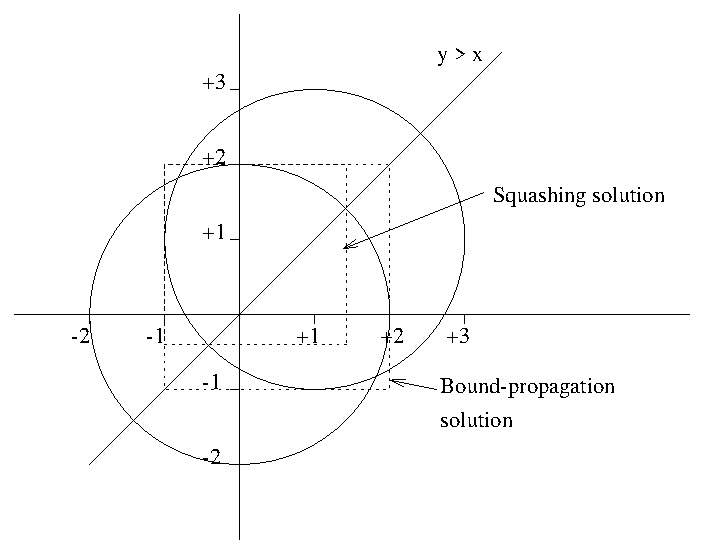
\includegraphics{example1.eps}
\caption{Propagation with Squash algorithm (example)}
\end{figure}

All points (X,Y) Y $>$= X, lying within the intersection of 2 circles with
radius 2, one centred at (0,0) the other at (1,1).
\begin{quote}
\begin{verbatim}
[eclipse 2]: 4 $>= X^2 + Y^2, 4 $>= (X-1)^2+(Y-1)^2, Y $>= X.

Y = Y{-1.0000000000000004 .. 2.0000000000000004}
X = X{-1.0000000000000004 .. 2.0000000000000004}

Delayed goals:
    ...
yes.
\end{verbatim}
\end{quote}
The bound-consistency solution does not take into account the X $>$= Y
constraint. Intuitively this is because it passes through the corners
of the box denoting the solution to the problem of simply intersecting
the two circles.

\begin{quote}
\begin{verbatim}
[eclipse 2]: 4 $>= X^2 + Y^2, 4 $>= (X-1)^2+(Y-1)^2, Y $>= X,
                squash([X,Y], 1e-5, lin).

X = X{-1.0000000000000004 .. 1.4142135999632601}
Y = Y{-0.41421359996326 .. 2.0000000000000004}

Delayed goals:
    ...
yes.
\end{verbatim}
\end{quote}

\subsection{Obtaining Solver Statistics}

(Using the facilities described in this section requires importing the
\bipref{ic_kernel}{../bips/lib/ic_kernel/index.html} module.  Also, since
they depend on the internals of the IC library, the details presented here
are subject to change without notice.)

Often it is difficult to know where the solver spends its time.
The library has built-in counters which keep track of the number of times
various events occur:
\begin{description}
    \item[ic_lin_create]
	The number of linear constraints set up.
    \item[ic_lin_prop]
	The number of times a linear constraint is propagated.
    \item[ic_uni_prop/ic_bin_prop/ic_tern_prop]
	The number of times a non-linear (unary/binary/ternary) operator is
	propagated.
    \item[ic_split]
	The number of domain splits in locate/2,3,4.
    \item[ic_squash]
	The number of squash attempts in squash/3 or locate/4.
\end{description}

Users who wish to track activity within their own programs may (if they
wish) use the same mechanism.  New event types can be registered (see
below) and actions recorded by calling the
\biptxtref{ic\_event(Event)}{ic_event/1!ic_kernel}{../bips/lib/ic_kernel/ic_event-1.html}
predicate.

The counters are controlled using the primitives:
\begin{description}
\item[\biptxtref{ic\_stat(on)}{ic_stat/1!ic_kernel}{../bips/lib/ic_kernel/ic_stat-1.html}]
\item[\biptxtref{ic\_stat(off)}{ic_stat/1!ic_kernel}{../bips/lib/ic_kernel/ic_stat-1.html}]
Enables/disable collection of statistics.  Default is off.

\item[\biptxtref{ic\_stat(reset)}{ic_stat/1!ic_kernel}{../bips/lib/ic_kernel/ic_stat-1.html}]
Reset statistics counters.

\item[\biptxtref{ic\_stat(print)}{ic_stat/1!ic_kernel}{../bips/lib/ic_kernel/ic_stat-1.html}]
Print statistics counters to the standard output stream.

\item[\biptxtref{ic\_stat_get(-Stat)}{ic_stat_get/1!ic_kernel}{../bips/lib/ic_kernel/ic_stat_get-1.html}]
Returns a list of CounterName=CounterValue pairs, summarising the
computation since the last reset.

\item[\biptxtref{ic\_event(+Name)}{ic_event/1!ic_kernel}{../bips/lib/ic_kernel/ic_event-1.html}]
Records the fact that the named event has happened.

\item[\biptxtref{ic_stat\_register\_event(+Name,+Description)}{ic_stat_register_event/2!ic_kernel}{../bips/lib/ic_kernel/ic_stat_register_event-2.html}]
Registers a new event type and sets the counter to 0.  This allows
user-defined predicates to record their own events within the same
framework.

\end{description}


\section{General Guidelines for the Use of the IC library}
Whilst IC has been designed to provide a flexible, consistent and yet
powerful framework for many sorts of constraint satisfaction
problems, it can not be all things to all people.

There are circumstances under which IC will not propagate all possible
information, for reasons of efficiency.

It is the purpose of this section to point out ways that may help IC
to solve problems more efficiently.

Typical constraint satisfaction problems are solved by iteratively
propagating information from basic constraints until no more
propagation can take place (i.e.\ a fixed point has been reached), and
then reducing the domain of a variable so as to prompt more
propagation.

As with most constraint solvers the propagation provided by the
builtin constraints is rarely able to solve large problems completely
without the need for some form of search.  A number of factors affect
the speed of the propagation phase.

\begin{enumerate}
\item The size of the initial domains.
Smaller domains typically result in propagation reaching a fixed point
sooner.  So give explicit initial domains to as many variables as possible.
\item Integer domains allow more propagation.
An important point to note here is that (as in mathematics) IC treats
integers as a strict subset of the reals, and as such the integer
domain \verb|0 .. 100| contains significantly fewer values than the
real domain \verb|0.0 .. 100.0|.  With this in mind, IC attempts to
infer integrality where possible (e.g.\ the sum of two integer variables
is constrained to be integer), however integer domains (where
applicable) should be used in user code.

The difference becomes apparent when dealing with strict inequalities, for example.
\begin{verbatim}
[eclipse 4]: reals([X]), X $> 5.

X = X{5.0 .. 1.0Inf}


Delayed goals:
        ic : (X{5.0 .. 1.0Inf} > 5)
Yes (0.00s cpu)
\end{verbatim}
Note that the lower bound of X is still five despite the fact that X
has been constrained to be strictly greater than five.  Further note
the presence of a delayed goal which will fail should X be constrained
to be exactly five.

\begin{verbatim}
[eclipse 5]: integers([X]), X $> 5.

X = X{6 .. 1.0Inf}
Yes (0.00s cpu)
\end{verbatim}
In this example since X is known to be integral, the lower bound of X
can be set to 6, as there are no integers between five and six.
\end{enumerate}


\section{User defined constraints}

The library \bipref{ic_kernel}{../bips/lib/ic_kernel/index.html} provides a
number of facilities useful for implementing IC constraints or otherwise
extending the facilities provided by the standard IC library.

While the \bipref{ic_kernel}{../bips/lib/ic_kernel/index.html} library
exposes the structure of the IC attribute to the programmer (see below),
accessing it directly is strongly discouraged (if for no other reason,
the internals of IC may continue to evolve).
For accessing information about a variable and its domain, use the
predicates described earlier in section~\ref{domain-query} ``Variable query
predicates''.
For modifying a variable, it is particularly important to go through the
access predicates, in order to make sure that the internal state remains
consistent, that appropriate constraints are scheduled for execution as a
result of the change, etc.
The predicates available for modifying a variable are discussed in the next
section.

\subsection{Modifying variable domains}

When using IC variables in normal code, one would typically use the
\verb|$\=|, \verb|$=<| and \verb|$>=| family of constraints to (resp.)
remove a value, reduce the upper bound or increase the lower bound of a
variable.

While these constraints are good for normal CSP solving, they have a
number of properties which may be less desirable when writing new
constraints.  In particular, they may leave unwanted delayed goals
behind and may perform extra propagation before returning (it may be
desirable to perform all required bound updates before allowing further
propagation to occur).

To give the constraint writer more control over such matters, special
predicates exist in the \bipref{ic_kernel}{../bips/lib/ic_kernel/index.html}
module which allow direct modification of the domain without the waking of
goals (they are scheduled for execution but not actually executed).
These predicates generally accept an IC variable, a non-IC variable (which
will be constrained to make it a real IC variable) or a number.

Full details on these predicates can be found in the reference manual; they
are listed here for completeness.  Note that with the exception of
\bipref{impose_bounds/3}{../bips/lib/ic_kernel/impose_bounds-3.html} none of
the goals call \bipref{wake/0}{../bips/kernel/suspensions/wake-0.html}, so
the programmer is free to do so at a convenient time.

\begin{description}
\item[\bipref{impose_min/2}{../bips/lib/ic_kernel/impose_min-2.html}]
Set the lowerbound.
\item[\bipref{impose_max/2}{../bips/lib/ic_kernel/impose_max-2.html}]
Set the upperbound.
\item[\bipref{impose_bounds/3}{../bips/lib/ic_kernel/impose_bounds-3.html}]
Sets both upper and lower bounds.
\item[\bipref{exclude/2}{../bips/lib/ic_kernel/exclude-2.html}]
Excludes an integer from an integral variable.
\item[\bipref{exclude_range/3}{../bips/lib/ic_kernel/exclude_range-3.html}]
Excludes a range of integers from an integral variable.
\item[\bipref{set_var_type/2}{../bips/lib/ic_kernel/set_var_type-2.html}]
Makes the variable be of the given type.
\item[\bipref{set_vars_type/2}{../bips/lib/ic_kernel/set_vars_type-2.html}]
Like set_var_type, but works for lists and submatrices of variables as well.
\end{description}

\subsection{The IC attribute}

The IC attribute is a meta-term which is attached to all variables which
take part in IC constraints.
\bipref{ic_kernel}{../bips/lib/ic_kernel/index.html} defines the IC
attribute as a structure of the following form:
\begin{verbatim}
ic{var_type:Type,
         lo:Lo,
         hi:Hi,
         bitmap:Bitmap,
         min:SuspMin,
         max:SuspMax,
         hole:SuspHole,
         type:SuspType
        }
\end{verbatim}


This structure holds:

\begin{description}
\item[var_type] The type of the variable.  This defaults to 'real' but may
become 'integer' after an explicit call to {\bf integers/1}, by being
included in an integer constraint (e.g.\ {\bf \#=}) or by inferences made
during constraint propagation.
\item[lo] The lower bound of the variable's domain, as a float.
\item[hi] The lower bound of the variable's domain, as a float.
\item[bitmap] Where relevant, a bitmap representation of the integer domain;
where not relevant it holds the atom \verb|undefined|.
\item[min] Suspension list of goals to be woken on lower bound changes.
\item[max] Suspension list of goals to be woken on upper bound changes.
\item[hole] Suspension list of goals to be woken when a value is removed
from the middle of a domain.  Such removals only happen for integer
variables whose domain is finite.
\item[type] Suspension list of goals to be woken when a variable's type
becomes more constrained, i.e.\ when a variable goes from being real to
being integer.
\end{description}

The suspension list names can be used in
\bipref{suspend/3}{../bips/kernel/suspensions/suspend-3.html} and
related predicates to denote an appropriate waking condition.

The attribute of a domain variable can be accessed with the predicate
\bipref{get_ic_attr/2}{../bips/lib/ic_kernel/get_ic_attr-2.html}.

As noted above, direct access and manipulation of the attribute is
discouraged; use the access predicates instead.

\index{library!ic|)}

%HEVEA\cutend

